\section{Implementation}
This chapter describes the implementation of the correction algorithm as 
realized in Version 1.0.0 of \cite{OMC-TeamIRNLRDTCorrection}.
Direct links to lines of the code as well as usage of \ttt{python} is avoided,
yet the structure and naming of the sections in this chapter follows is kept close to the names in the actual code,
which can be found on
\href{https://github.com/pylhc/irnl_rdt_correction}{https://github.com/pylhc/irnl\_rdt\_correction}.
The API is documented in  
\href{https://pylhc.github.io/irnl_rdt_correction}{https://pylhc.github.io/irnl\_rdt\_correction}.

\begin{important}
        \item[\color{CernRed} Attention] While this note follows the convention of \textbf{n = 1 for dipole fields}, 
        in the code the \ttt{MAD-X} convention of \textbf{n = 0 for dipole fields}  is used, as the input will already be in that format.
\end{important}

\myparagraph{Dependencies}

The package is mostly self-contained and depends only on:

\begin{options}
        \item[numpy]
        provides an easy way to work with numerical data in arrays as well as additional functionality 
        e.g. for solving linear equation systems~\cite{HarrisArrayProgrammingNumPy2020}.
        \item[pandas]
        allows working with data-tables, which are used to structure the data and allow easy access and identification 
        of the different optics parameters~\cite{pandas}.
        \item[tfs-pandas]
        a wrapper for \opt{pandas} to read tables from  and write tables into files of 
        the Table File System (TFS) format used by \ttt{MAD-X}~\cite{CERNMadX}~\cite{OMC-TeamTFSPandas}.
\end{options}


\subsection{Beam Directions}
\label{sec:BeamDirection}

\begin{figure}[h!]
    \centering
    \begin{subfigure}{0.4\textwidth}
        % 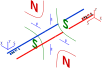
\includegraphics[width=\textwidth]{beamDirection/quadBeam1.png}
        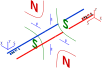
\includegraphics[width=\textwidth]{beamDirection/quadBeam1.pdf}
        \caption{In reference frame of Beam~1}
    \end{subfigure}
    \hspace{2em}
    \begin{subfigure}{0.4\textwidth}
        % 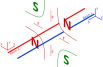
\includegraphics[width=\textwidth]{beamDirection/quadBeam2.png}
        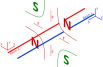
\includegraphics[width=\textwidth]{beamDirection/quadBeam2.pdf}
        \caption{In reference frame of Beam~2}
    \end{subfigure}
    \caption{Schematic of two beams traveling in opposite directions through a quadruople.}
    \label{fig:BeamDirection}
\end{figure}

Because of the opposite traveling direction of Beam~2, magnetic fields in the reference frame of this beam look as if rotated
by $\qty{180}{\degree}$ around the y-axis at the center of the magnet, compared to the reference frame of Beam~1.
Hence magnets with y-axis symmetry will have the same effect on the beams, 
while magnets that do not have this symmetry will look like they have opposite-sign fields,
e.g. a focusing quadrupole magnet with strength $K_2$ in Beam~1 is seen as a defocusing magnet with $-K_2$ in Beam~2 
(see \cref{fig:BeamDirection}).
%
In general:
%
\begin{equation}
\label{eq:B1toB2}
(K_n + iJ_n)^\text{B2} =
\begin{cases}
        (-K_n + iJ_n)^\text{B1} \; , \text{if } n \text{ is even} \\
        (\phantom{-}K_n - iJ_n)^\text{B1} \; , \text{if } n \text{ is odd} \;.
\end{cases}
\end{equation}
%
This does not need to be taken into account as long as one stays within the reference frame of a single beam, 
as the physics (e.g. feed-down and RDTs) is symmetrical.
It becomes problematic when both beams are involved, especially as there are two different definitions for Beam~2 in \ttt{MAD-X}: 
One called is ``Beam~2'', for which all elements are defined in the reference frame of Beam~1 
and the beam direction is handled via a negative beam velocity (\ttt{BV=-1}); 
the other one is called ``Beam~4'' and here the whole lattice is inverted and the beam travels in forward direction (\ttt{BV=1}),
which means the field strengths follow the relation in \cref{eq:B1toB2}.
Of further confusion is the fact, that the beam direction is already taken into account in the field strength data of \ttt{TWISS} 
in \ttt{MAD-X}, but not in the \opt{errors} output of \ttt{ESAVE} and not in the horizontal orbit, the \ttt{X} and \ttt{DX} data respectively.
To assure consistent behaviour, the optics of ``Beam~2'' are brought into the reference frame of ``Beam~4'' upon loading.

When building an equation system as in \cref{eq:linearEqSystemDoubleOptics}, the reference frame needs again to be taken into account:
\Cref{eq:linearEqSystemDoubleOptics} is only correct, when all values are calculated in the same reference frame.  
Yet they are not.
Each line  of  is correct in its own reference frame, but the $K_nL$ and $J_nL$ values are shared in between them. 
To account for the appropriate signs, the signs of the coefficients are inverted according to \cref{eq:B1toB2} where needed for Beam~2: 
%
\begin{equation}    
    \label{eq:linearEqSystemDoubleOpticsBeamDirection}
    \begin{split}
        \begin{pmatrix}
            b_{jklm}^{(cl, \text{B1})} & b_{jklm}^{(cr, \text{B1})} \\
            \pm b_{jklm}^{(cl, \text{B2})} & \pm b_{jklm}^{(cr, \text{B2})}
        \end{pmatrix}
        \begin{pmatrix}
            K_{n}L_{cl} \\ 
            K_{n}L_{cr}
        \end{pmatrix}
        = -
        \begin{pmatrix}
            I^{(\text{B1})}_{jklm} \\ 
            I^{(\text{B2})}_{jklm} 
        \end{pmatrix} 
        \quad \text{if} \; n \; \text{is} \; \{\substack{\text{odd}\\\text{even}} \;,
        \\ 
        \begin{pmatrix}
            ib_{jklm}^{(cl, \text{B1})} & ib_{jklm}^{(cr, \text{B1})} \\
            \pm ib_{jklm}^{(cl, \text{B2})} & \pm ib_{jklm}^{(cr, \text{B2})}
        \end{pmatrix}
        \begin{pmatrix}
            J_{n}L_{cl} \\ 
            J_{n}L_{cr}
        \end{pmatrix}
        = -
        \begin{pmatrix}
            I^{(\text{B1})}_{jklm} \\ 
            I^{(\text{B2})}_{jklm} 
        \end{pmatrix} 
        \quad \text{if} \; n \; \text{is} \; \{\substack{\text{even}\\\text{odd}} \;.
    \end{split}
\end{equation}
%
Calculating the corrector strengths in this way also allows for easy setting of the \ttt{MAD-X} knobs
to set the corrector strengths, as these are defined with positive sign in the lattice sequence of Beam~1 (and ``Beam~2'')
and negative sign in the lattice sequence of ``Beam~4''.
On the other hand, when updating the optics tables itself, e.g. to correct feed-down from the correctors, 
the original signs need to be recovered for ``Beam~2'' and ``Beam~4''.

This is the way the beam direction is currently implemented in the code.
Where this sign change is applied, it will be explicitly mentioned again in the following chapters.

\begin{important}
        \item[\raisedtaget{Hint:SwitchBeamSigns}\color{AtlasGreen} Hint]
        Another option would be to bring everything into the reference frame of Beam~1 in the first place, 
        i.e. switching the signs of the ``Beam~4'' $K_nL$ and $J_nL$ according to \cref{eq:B1toB2}, 
        in \opt{twiss} and \opt{errors}, as well as the same $K_nL, J_nL$ in the \opt{twiss} of ``Beam~2''.
        It still needs to be shown, that in this case feed-down is correctly calculated, 
        as the direction of the beam is no longer taken into consideration.
        If this is shown, all beam related sign changes in the code, but the initial one to bring 
        as described just now upon loading \opt{twiss} and \opt{errors}, could be removed.
        See also \cref{sec:Todo}.
\end{important}

% \newpage
\subsection{Main}
The entry-point to run the corrections is the \ttt{irnl\_rdt\_correction()} function in \\
\ttt{irnl\_rdt\_correction/main.py}.


\subsubsection{Preparations}
\label{sec:Preparations}

\myparagraph{Check Opts}
First the \ttt{options} given by the user are validated and default values set.
These options are:
\begin{options}
        \item[twiss] the optics of the machine as given by the \ttt{TWISS} command in \ttt{MAD-X}.
                     \textbf{Important:} All of these elements are used for correction. 
                     They are assumed to follow the LHC naming scheme, so that they can be split into IRs, 
                     but to limit the correction to only calculate the effective RDT over certain IR elements,
                     these need to be filtered \textbf{beforehand}, e.g. in \ttt{MAD-X}.
        \item[errors] errors on the optics of the machine, 
                      as given by the \ttt{ESAVE} command in \ttt{MAD-X}.
                      All elements of \opt{errors} need to be present in \opt{twiss},
                      but elements not present in \opt{errors} are assumed to have zero errors.
        \item[beam] the beam the optics come from, definition as in \ttt{MAD-X}: 1, 2 or 4.
        \item[output] path to write the results into (as table and as \ttt{MAD-X} commands.)
        \item[rdts] a set of RDTs, defined either like $f_{jklm}$ ($f_{jklm*}$) as strings of format
                    \ttt{"fjklm"} (\ttt{"fjklm*"}) to correct
                    these RDTs (RDTs with switched $\beta$, see \cref{eq:effectiveRDT*}) 
                    by the correctors of their order and orientation.
                    Alternatively they can be given as a dictionary, with the RDTs as keys
                    and a list of corrector fields (e.g. $b_4$) as strings (e.g. \ttt{"b4"}) 
                    as values to specify which correctors to use to correct this RDT \cref{eq:linearEqSystemSingle}. 
                    If the order of the corrector is higher than the order of the RDT, its feed-down
                    is used to correct the RDT. If the order is lower, an error is raised.
                    If \opt{rdts2} is given, these apply only \ttt{MAD-X} to the first optics. 
                    (Default depends on \opt{accel})
        \item[rdts2] same format as \opt{rdts}, but the given RDTs are used to correct the second optics.
                     If only \opt{rdts} is given, they apply to all optics.
        \item[accel] The name of the accelerator to use. \ttt{"lhc"} and \ttt{"hllhc"} are implemented.
                     This determines the default RDTs to use, as well as the correct names for the correctors
                     in the lattice. (Default: \ttt{"lhc"})
        \item[feeddown] maximum order of the feed-down to include, i.e. $Q$ in \cref{eq:feeddownOrderN}. 
        \item[ips] a list of integers of the IPs to correct. (Default: 1,2,5,8)
        \item[solver] solver to use to solve the built linear equation system. 
                      Can be one of \ttt{"lstsq"}, \ttt{"inv"} or \ttt{"linear"}.  (Default \ttt{"lstsq"}).
        \item[update\_optics] if this option is set to \ttt{True}, the correction begins with the highest 
                              order and the newly calculated corrector strengths are inserted into the optics 
                              for the following so that feed-down from these correctors can be taken into account.
                              Necessary for accurate corrections in case $Q \geq 0$ (as set via \opt{feeddown}).
                              (Default: \ttt{True})
        \item[ignore\_corrector\_settings] if this is \ttt{False}, the corrector values of the
                                          optics are used as initial conditions. Otherwise they are ignored.
                                          (Default: \ttt{False})
        \item[ignore\_missing\_columns] if \ttt{True} missing strength columns in any of the input files are assumed
                                        to be zero, instead of raising an error.
                                        (Default: \ttt{False})
        \item[iterations] (re-)iterate correction, starting with the previously
                          calculated values. Needs to be $> 0$, as the first calculation
                          counts as an iteration.
                          (Default: 1)
\end{options}
%
The default RDTs for the LHC and HL-LHC are as in the original triplet correction scripts \cite{FartoukhLHCNonlinearTriplet2008,FartoukhHLLHCNonlinearTriplet2012}:
%
\begin{table}[h]
        \centering
        \caption{Default RDTs used in the correction script if 
                \ttt{rdts} option is not provided.}
        \label{tab:defaultRDTs}
        \begin{tabular}{clll}
        \toprule
        \midrule
        \opt{accel} & \multicolumn{2}{c}{RDTs} & \multicolumn{1}{c}{description}\\
        \midrule
             \ttt{"lhc"}
            & \ttt{"F0003"}& \ttt{"F0003*"}& correct $a_3$ errors with $f_{0003}$\\
            &\ttt{"F1002"}& \ttt{"F1002*"}& correct $b_3$ errors with $f_{1002}$\\
            &\ttt{"F1003"}& \ttt{"F3001"}& correct $a_4$ errors with $f_{1003}$ and $f_{3001}$\\
            &\ttt{"F4000"}& \ttt{"F0004"}& correct $b_4$ errors with $f_{4000}$ and $f_{0004}$\\
            &\ttt{"F6000"}& \ttt{"F0006"}& correct $b_6$ errors with $f_{6000}$ and $f_{0006}$\\
         \midrule
            \ttt{"hllhc"}
              &\ttt{"F0003"}& \ttt{"F0003*"}& correct $a_3$ errors with $f_{0003}$\\
              &\ttt{"F1002"}& \ttt{"F1002*"}& correct $b_3$ errors with $f_{1002}$\\
              &\ttt{"F1003"}& \ttt{"F3001"}& correct $a_4$ errors with $f_{1003}$ and $f_{3001}$\\
              &\ttt{"F0004"}& \ttt{"F4000"}& correct $b_4$ errors with $f_{0004}$ and $f_{4000}$\\
              &\ttt{"F0005"}& \ttt{"F0005*"}& correct $a_5$ errors with $f_{0005}$\\
              &\ttt{"F5000"}& \ttt{"F5000*"}& correct $b_5$ errors with $f_{5000}$\\
              &\ttt{"F5001"}& \ttt{"F1005"}& correct $a_6$ errors with $f_{5001}$ and $f_{1005}$\\
              &\ttt{"F6000"}& \ttt{"F0006"}& correct $b_6$ errors with $f_{6000}$ and $f_{0006}$\\               
        \bottomrule
        \end{tabular}
\end{table}


\myparagraph{Sort RDTs}
\label{par:SortRDTs}

The input RDTs are then transformed into \ttt{RDT}-objects, which contain information about their order $n = j + k + l + m$, 
their skewness ($l + m  \equiv  1 \mod 2$) and wether they should be calculated with swapped $\beta$-exponents (if given by the \ttt{*} in the name).
A mapping is then produced to the desired correctors these RDTs should be corrected with, 
resulting in a dictionary of \texttt{RDT}-objects and sequences of strings, defining corrector orientation and order (e.g. \ttt{"b4"}).
The latter are either taken from the user input parameters, or if not given, determined by the RDT itself.
This mapping is then sorted by highest RDT order and (arbitrarily) skew before normal.

\myparagraph{Get Orders}
\label{par:GetOrders}

Now, the feed-down orders are checked. 
It is for example not possible to update the optics in a useful manner, if two orders of feed-down are required and
a normal octupole RDT ($b_4$) should be corrected by feed-down from a normal dodecapole corrector ($b_6$), 
while at the same time a normal decapole RDT ($b_5$) needs to be corrected by a corrector of the same order.
As the $b_5$ RDT is corrected before the $b_4$ RDT, the $b_6$ corrector is still unassigned and its feed-down cannot 
be taken into account when calculating the $b_5$ correction.
This issue could be overcome by sorting not by highest RDT order but by highest corrector order per RDT, 
which is implemented but has yet to be tested (see~\cref{sec:Todo}).

It is also checked, wether the field order of a given corrector is lower than the order of its RDT, 
as in this case the corrector can have no influence on the effective RDT (as they are RDTs of first order in field strengths).
In this case an error is thrown.

Also the \ttt{needed orders} are evaluated, which are the field orders needed in the optics to calculate all desired 
effective RDTs with the requested \opt{feeddown}.


\myparagraph{Load Optics}

If the \opt{twiss} and \opt{errors} are not given as \opttarget{tfs-pandas}{TfsDataFrames} already, they are then read in.
It is checked that the number of \opt{twiss} and \opt{errors} tables given equals.
The contents of the tables themselves are checked for the presence of elements, 
e.g. elements in \opt{errors} need to be present in \opt{twiss}, as their position and $\beta$-functions need to be known. 
Elements not found in \opt{errors}, which are present in \opt{twiss} are added with zero values.
It is then also checked if all \ttt{needed orders} as determined in the previous step are present in the \ttt{KNL} and \ttt{KNSL} columns of the
\ttt{TfsDataFrames}. Depending on the choice of \opt{ignore\_missing\_columns} they are either filled with zeros or the program ends with an error.

At this point, the beam direction is also taken care of, i.e. if \opt{twiss} and \opt{errors} of \ttt{MAD-X}' ``Beam~2'' are given, 
the horizontal orbit columns in both (\ttt{X} and \ttt{DX}) will switch sign, as well as all strengths of magnets, 
that are not symmetric on beam direction change, or \textit{anti mirror-symmetric} as it is called in the code.
In this manner, the optics of ``Beam~2'' are brought into the reference frame of ``Beam~4''.
See \cref{sec:BeamDirection} for details.

For convenience, the loaded optics are then stored in a sequence of \ttt{Optics}-objects, 
each containing single instance of the given \opt{beam}, \opt{twiss} and \opt{errors}. 


\subsubsection{Build and Solve Equation System}
The core of the correction algorithm is the building and solving of the equation system \cref{eq:linearEqSystemSingle}
and extending it for multiple RDTs (\cref{eq:linearEqSystemDouble}), 
beam optics (\cref{eq:linearEqSystemDoubleOptics} and \cref{eq:linearEqSystemDoubleOpticsBeamDirection}), 
but also possibly solving for multiple correctors at a time when correcting via feed-down (\cref{eq:linearEqSystemFeeddown}).

\myparagraph{Get RDT Maps grouped by Correctors}
To increase numerical stability and also allow to incorporate feed-down from correctors to lower order RDTs, 
not all corrector strengths are calculated at the same time, but many independent equation systems are build, 
and solved consecutively.

To achieve this, the RDTs to correct are grouped by common correctors: 
The correctors of the first RDT, as given by the built RDT map in \cref{par:SortRDTs} in \cref{sec:Preparations}, 
are used to find other RDTs sharing these correctors, the correctors of which are then used to determine which other RDTs
need to be corrected together, until all remaining RDTs have no correctors in common with the selected ones.
The grouping is done for all given optics at the same go, so that also common correctors are found between them.

After solving the equation system for the currently selected RDTs, the process of grouping RDTs is repeated with the remaining RDTs
until none are left. 
As this algorithm for grouping is not straightforward, details about the actual implementation are found directly in the comments of the code.

\myparagraph{Get available Correctors}
\label{par:GetAvailableCorrectors}
In a loop over the given \opt{ips}, the so far abstract corrector names, identifying only orientation and order of the correctors, 
are now instancialized as \ttt{Corrector}-objects by finding the appropriate correctors for the current IP in the \ttt{Optics}.
The current implementation is very (HL-)LHC specific, as it uses the naming scheme, depending on the given \opt{accel}.
If correctors are present in only one of the given \ttt{Optics}, but not in the other, an \ttt{EnvironmentError} is raised.
When only one of the two correctors per side is present, a \ttt{warning} is printed, and if no matching corrector for this IP is found
in the optics, this \ttt{info}rmation is logged and the corrector not included in the correction of this IP.

The corrector values are initialized in accordance with \opt{ignore\_corrector\_settings} (they are initialized as zero, or as given in the optics)
and saved in case they need to be restored later (\opt{update\_optics} = \ttt{False}).
This is important, as the algorithm actually calculates the \textit{change in corrector strength} needed to compensate the RDT, as explained in the next paragraph.

\myparagraph{Build Equation System}
\label{par:BuildEquationSystem}
The equation system for the current RDTs, correctors and optics including the desired feed-down
(\cref{eq:linearEqSystemSingle,eq:linearEqSystemDouble,eq:linearEqSystemDoubleOptics,eq:linearEqSystemDoubleOpticsBeamDirection,eq:linearEqSystemFeeddown})
for the current IP, e.g.
%
\begin{equation}    
    \label{eq:linearEqSystemFull}
    \newcommand{\ipbo}{\text{IP1,B1}}
    \newcommand{\ipbt}{\text{IP1,B2}}
        \begin{pmatrix}
            b_{jklm}^{(cl,\ipbo)} & b_{jklm}^{(cr,\ipbo)} & b_{jklm,p}^{(cl,\ipbo)} & b_{jklm,p}^{(cr,\ipbo)} & \cdots \\
            b_{jklm}^{(cl,\ipbt)} & b_{jklm}^{(cr,\ipbt)} & b_{jklm,p}^{(cl,\ipbt)} & b_{jklm,p}^{(cr,\ipbt)} & \cdots \\
            b_{j'k'l'm'}^{(cl,\ipbo)} & b_{j'k'l'm'}^{(cr,\ipbo)} & b_{j'k'l'm',p}^{(cl,\ipbo)} & b_{j'k'l'm',p}^{(cr,\ipbo)} & \cdots
        \end{pmatrix}
        \begin{pmatrix}
            \Delta K_{n}L_{cl} \\ 
            \Delta K_{n}L_{cr} \\
            \Delta K_{n+p}L_{cl} \\ 
            \Delta K_{n+p}L_{cr} \\ 
            \vdots
        \end{pmatrix}
        = - 
        \begin{pmatrix}
            I_{jklm}^{(\ipbo)} \\ 
            I_{jklm}^{(\ipbt)} \\ 
            I_{j'k'l'm'}^{(\ipbo)} \\ 
            \vdots 
        \end{pmatrix} \, ,
\end{equation}
%
is now build.
In contrast to \cref{eq:equationSum}, the integrals $I_{jkml}$ on the rhs of \cref{eq:linearEqSystemFull} 
contains also the corrector settings as currently in the \ttt{Optics}. 
For this reason, the $\Delta K_nL$ values are introduced here, which allow to solve and update this equation system
as often as given in \opt{iterations} to improve upon in a next step.
 

\myparagraph{Solve Equation System and update Values}
\label{par:SolveEquationSystem}

The built linear equation system is now solved with one of the standard solvers, as given by via the option \opt{solver}.
\ttt{"inv"} and \ttt{"linear"} refer hereby to inverting the coefficient matrix on the lhs of \cref{eq:linearEqSystemFull} 
and performing a dot-product with the rhs and to solving it directly via \opt{numpy}'s \ttt{solve} method, respectively.
These are only implemented for testing and debugging purposes and should not be used in real applications as they are inefficient
and work only with well-determined matrix equations.
The default method \ttt{"lstsq"} makes use of the \opt{numpy} method of the same name and performs a linear least-squares optimization
and works on under-, well-, or over-determined equation systems.

As explained above the resulting values are the changes to the current corrector values, 
which are now applied and used to update the optics and the integrals on the rhs of \cref{eq:linearEqSystemFull} are
recalculated, informing about the change in the effective RDTs and to be used in the next \opt{iteration}, if there will be one. 

After the \opt{iteration}s for the current IP have been run,
the original corrector values will be restored, if they had been saved (see~\cref{par:GetAvailableCorrectors}) 
and the corrections for the \opttarget{ips}{next given IP} is calculated.


\myparagraph{Output}
\label{par:Output}
After all corrector values have been calculated, they are finally written into \ttt{ASCII}-files, if \opt{outpath} is given, and returned 
in two different formats:
\begin{description}
  \item[As \ttt{MAD-X}] In this format the corrector names are converted into the circuit-knob-names as used in the lattice description in \ttt{MAD-X}.
                        As these refer to the non-integrated field strengths, the value is assigned by reference (\ttt{:=}) and divided by 
                        the lattice variable for the length of the corrector type (e.g. \ttt{l.MCTX}).
                        In this format, the correction can be immediately used in a \ttt{MAD-X} script.    
  \item[As \ttt{TfsDataFrame}] The second output format is a \ttt{DataFrame}, created from \ttt{IRCorrector}-objects. 
                        The attributes are mapped to the columns, while the different correctors are spread along the index.
                        The \ttt{DataFrame} is written out as a table in \ttt{TFS} format by \opt{tfs-pandas}.
\end{description}


\subsection{Tests}

A variety of tests has been deployed, testing the current status of the current implementation and 
trying to make the algorithm resilient against future bugs.
The tests are automatically run via github workflows and need to pass before any pull-request is 
accepted to the ``master''-branch of the repository.

Most tests cover certain specific ways to run the correction algorithm as a whole, 
while also some unit-tests have been implemented, where easily applicable.
To be able to validate the calculated corrections easily a non-physical \ttt{pseudo-model}
is created in most tests, with only a few of elements and arbitrary values for the parameters. 
For example, a constant $\beta$-function of $1$ can be used to simplify the equation systems and make them solvable by hand.
Currently running are tests for the following scenarios:

\begin{testlist}
\item[Standard Corrections] Test default correction capabilities.
    \begin{testlist}
        \item[Basic] Test the basic correction functionality and perform some sanity checks.
        Operates on a pseudo-model so that the corrector values are easily known.
        Sanity Checks:
        \begin{itemize}
            \item all correctors found
            \item correctors have the correct value (as set by errors or zero)
            \item all corrector circuits are present in the \ttt{MAD-X} script
        \end{itemize}
        \item[LHC Correction] Test LHC optics with random errors assigned.
        Sanity Checks:
        \begin{itemize}
            \item all correctors found
            \item correctors have a value
            \item all corrector circuits are present in the \ttt{MAD-X} script
        \end{itemize}
    \end{testlist}
\item[RDT Corrections] Test correction settings that are RDT specific.
    \begin{testlist}
        \item[Different RDTs] Test that different RDTs can be corrected and only their correctors
        are returned. Also checks that the corrector values are varying between RDTs
        when they should. Octupole RDTs are used for this example.
        \item[Switched Beta] Test using the special RDTs* where the beta-exponents are switched.
    \end{testlist}
\item[Dual Optics Corrections] Test the correction when giving more than one beam optics.
    \begin{testlist}
        \item[Dual Optics] Test that given two different optics an approximate solution will be found.
        \item[Dual Optics RDTs] Test calculations given two different optics and different RDTs.
    \end{testlist}
\item[Feed-Down Corrections] Test the feed-down calculation and correction.
    \begin{testlist}
        \item[General] Test feed-down functionality from decapoles to octupoles and sextupoles.
        \item[Correct via Feed-Down] Test correct RDT via feed-down from higher order corrector: 
        Use normal and skew deca- and dodecapole correctors to correct for normal octupole errors.
    \end{testlist}
\item[Unit-Tests] Test individual functions and classes.
    \begin{testlist}
        \item[Switch Signs] Test the sign-switching function from Beam~2 to Beam~4 (and that there is no switch given Beam~1 or Beam~4).
        \item[IRCorrector Class] Test the class representing IR Correctors
        \begin{itemize}
            \item instantiates
            \item has the right (in-)equalities 
            \item is sortable
            \item for different accelerators
        \end{itemize}
        \item[RDT Class] Test the class representing RDTs
        \begin{itemize}
            \item instantiates
            \item has the right (in-)equalities 
            \item is sortable
        \end{itemize}
    \end{testlist}
\end{testlist}

\subsection{To Do}
\label{sec:Todo}
\begin{important}
 \item[\color{AtlasGreen}easy] Allow not giving errors 
   (need to be \ttt{None} in the list or all \ttt{None}, 
   so that the list lengths are still the same and there is a
   clear correspondence twiss-errors-beams).
   They should then be assumed all zero.
 \item[\color{AtlasGreen}easy] Allow for more than two optics given
   (e.g. find corrections for 15cm and 30cm for both beams).
 \item[\color{AtlasOrange}medium] 
   Maybe sort RDTs by highest corrector instead of highest RDT order?
   This should allow for correctors that correct via feed-down
   to be assigned before lower order RDTs are calculated.
   It is already in the code, but commented out for now as
   might cause other problems. To be thought about and tested.
   See \cref{par:GetOrders} in \cref{sec:Preparations}.
 \item[\color{AtlasOrange}medium] 
   Consider switching the signs all into the reference frame of Beam 1.
   That means X, DX and anti-mirror-KN(S)L twiss and errors from Beam 4,
   and the anti-mirror-KN(S)L twiss from Beam 2.
   That should in principle allow to ignore all other beam-related sign switches.
   BUT: does this really work with all the feed-down options implemented
   (i.e. feed-down to RDT, feed-down from correctors)?
   It should, but needs to be checked and tested.
   See \hyperlink{Hint:SwitchBeamSigns}{\textcolor{AtlasGreen}{\textsc{\bfseries Hint}}} in \cref{sec:BeamDirection}.
 \item[\color{AtlasOrange}medium]
   Take phase advance between the elements and to the correction point at the entrance of the IR into account.
   That would mean correct the numerator of the \textit{actual} RDT (\cref{eq:RDTHamiltonianRelation}) instead 
   of the \textit{effective} RDT (\cref{eq:effectiveRDT}).
 \item[\color{CernRed}hard]
   Additionally to taking the phase-advance into account, one might try to optimize the actual RDTs at the position of the correctors.
   This might be very problematic, as we have two correctors (one on each side)
   per order, so that might become a non-linear problem (as now there
   are now two equations, one per corrector, which are non-linearly dependent.)
\end{important}
